\documentclass[11pt,oneside]{book}
\usepackage{amsmath}
\usepackage{amssymb}
\usepackage{amsthm}
\usepackage{amsfonts}
\usepackage{multirow}
\usepackage{float}
\usepackage{diagbox}
\usepackage{xcolor}
\usepackage{caption}
\usepackage{graphicx}
\graphicspath{{img/}}
\usepackage{paralist}
\usepackage{tikz}
\let\itemize\compactitem
\let\enditemize\endcompactitem
\let\enumerate\compactenum
\let\endenumerate\endcompactenum
\let\description\compactdesc
\let\enddescription\endcompactdesc
\setlength{\parindent}{0pt}
\title{Notes of Mathematical Analysis}
\author{}
\date{}
\newtheorem{theorem}{Theorem}[section]
\newtheorem*{lemma}{Lemma}
\newtheorem{definition}{Definition}[section]
\theoremstyle{definition}
\newtheorem{ex}{Exercise}[section]
\newtheorem*{answer}{Answer}
\newcommand\thmref[1]{\textbf{Theorem \ref{#1}}}
\newcommand\figref[1]{\textbf{Figure \ref{#1}}}
\begin{document}
\newtheorem*{tips}{\emph{TIPS}}
\chapter{Groups}
\section{Semigroups, monoids and groups}
\begin{ex}
    Give examples other than those in the text of semigroups and monoids that are not groups.
\end{ex}

\begin{answer}
    Semigroup: $(\mathbf{Z}_+, +)$

    Monoid: $(\mathbf{Z}_+, \times )$ 
\end{answer}

$$ $$

\begin{ex}
    Let $G$ be a group (written additively), $S$ a nonempty set, and $M(S,G)$ the set of all functions $f: S \rightarrow G$. Define addition in $M(S,G)$ as follows: $(f + g) : S \rightarrow G$ is given by $s \rightarrow f(s) + g(s) \in G$. Prove that $M(S,G)$ is a group, which is abelian if $G$ is.
\end{ex}

\begin{answer}
    Firstly we check $M(S,G)$ is a group
    \begin{enumerate}
        \item $f+g: s\to f(s) + g(s) \in G$, so $f+g\in M(S,G)$
        \item $(f+g)+h: s\to (f(s) + g(s)) + h(s)$, $G$ is a group, so $s\to (f(s) + g(s)) + h(s)\Leftrightarrow s\to f(s) + (g(s) + h(s))$, $(f+g)+h = f+(g+h)$.
        \item Take the unit element as $e': s\to e$. $f+e': s\to f(s)+ e'(s) =f(s)+e=f(s)$, so $f+e'=f$. Similarly, $e'+f = f$.
        \item For any $f\in M(S,G)$, take $f^{-1}: s\to (f(s))^{-1}$, whence $f(s)+(f(s))^{-1}=(f(s))^{-1}+f(s)=e$.
    \end{enumerate}
    In conclusion, $M(S,G)$ is a group. If $G$ is abelian $f+g: s\to f(s)+g(s)=g(s)+f(s)$, $f+g=g+f$, so $M(S,G)$ is abelian.
\end{answer}

$$ $$

\begin{ex}
    Is it true that a semigroup which has a left identity element and in which every element has a right inverse (see Proposition 1.3) is a group?
\end{ex}

\begin{answer}
    If $e$ is the left identity, $\forall a \in A, ea=a$ and $\forall a\in A ,\exists  a^{-1} s.t. aa^{-1}=e$. We have proved that if $cc=c$, then $c=e$. \[(a^{-1}a)(a^{-1}a)=a^{-1}(aa^{-1})a=a^{-1}(ea)=a^{-1}a\Rightarrow a^{-1}a=e\]
    $a^{-1}$ is also the left inverse. $ae=a(a^{-1}a)=(aa^{-1})a=ea=a$, $e$ is also the right identity.
\end{answer}

$$ $$

\begin{ex}
    Write out a multiplication table for the group $D_4^*$.
\end{ex}

\begin{answer}
    $D_4^*=\{R,R^{2}, R^{3},I,T_x,T_y,T_{13},T_{24}\}$
    \begin{table}[H]
        \centering
        \begin{tabular}{c|cccccccc}
        \multicolumn{1}{c}{} & $I$ & $R$ & $R^{2}$ & $R^{3}$ & $T_x$ & $T_y$ & $T_{13}$ & $T_{24}$  \\ 
        \cline{2-9}
        $I$ & $I$ & $R$ & $R^{2}$ & $R^{3}$ & $T_x$ & $T_y$ & $T_{13}$ &  $T_{24}$ \\
        $R$ & $R$ & $R^{2}$ & $R^{3}$ & $I$ & $T_{13}$ & $T_{24}$ & $T_y$ & $T_x$  \\
        $R^{2}$ & $R^{2}$ & $R^{3}$ & $I$ & $R$  & $T_y$ & $T_x$ & $T_{24}$ & $T_{13}$  \\
        $R^{3}$ & $R^{3}$ & $I$ & $R$  & $R^{2}$ & $T_{24}$ & $T_{13}$ & $T_x$ & $T_y$  \\
        $T_x$ & $T_x$ & $T_{24}$ & $T_y$ & $T_{13}$ & $I$ & $R^{2}$ & $R^{3}$ & $R$  \\
        $T_y$ & $T_y$ & $T_{13}$ & $T_x$ & $T_{24}$ & $R^{2}$ & $I$ & $R$ & $R^{3}$  \\
        $T_{13}$ & $T_{13}$ & $T_y$ & $T_{24}$ & $T_x$ & $R^{3}$ & $R$ & $I$ &  $R^{2}$ \\
        $T_{24}$ & $T_{24}$ & $T_x$ & $T_{13}$ & $T_y$ & $R$ & $R^{3}$ & $R^{2}$ &  $I$
        \end{tabular}
        \end{table}
\end{answer}

$$ $$

\begin{ex}
    Prove that the symmetric group on $n$ letters, $S_n$, has ordrer $n!$.
\end{ex}

\begin{answer}
    For a set $A$ whose order is $n$, we prove there's $n!$ different bijections by induction
    \begin{enumerate}
        \item For $n=1$, trivial.
        \item Assume $n=k$, there's $k!$ bijections. For $n=k+1$m fix one element in $A$, and take $a\to a$, there's $k$ free elements, so there's $K!\cdot(k+1)$ bijections in total.
    \end{enumerate}
    By induction, we get the result.
\end{answer}

$$ $$

\begin{ex}
    Write out an addition table for $Z_2\oplus Z_2$. $Z_2\oplus Z_2$ is called the Klein four group.
\end{ex}

\begin{answer}
    $Z_2=\{1,0\}$, $Z_2\oplus Z_2=\{(1,1), (1,0), (0,1), (0,0)\}$
    \begin{table}[H]
        \centering
        \begin{tabular}{c|cccc}
            \multicolumn{1}{c}{} & $(1,1)$ & $(1,0)$ & $(0,1)$ & $(0,0)$\\
            \cline{2-5}
            $(1,1)$ & $(0,0)$ & $(0,1)$ & $(1,0)$ & $(1,1)$ \\
            $(1,0)$ &$(0,1)$  & $(0,0)$ & $(1,1)$ & $(1,0)$ \\
            $(0,1)$ & $(1,0)$ & $(1,1)$ & $(0,0)$ & $(0,1)$ \\
            $(0,0)$ & $(1,1)$ & $(1,0)$ & $(0,1)$ & $(0,0)$
        \end{tabular}
    \end{table}
\end{answer}

$$ $$

\begin{ex}
    If $p$ is prime, then the nonzero elements of $Z_p$ form a group of order $p - 1$ under multiplication. Show that this statement is false if $p$ is not prime.
\end{ex}

\begin{answer}
    For the set $Z_p\backslash\{\bar{0}\}$
    \begin{enumerate}
        \item $Z_p\backslash\{\bar{0}\}$ is obviously associative and communicative.
        \item Take $\bar{1}$ as the identity element, $\forall \bar{a}\in Z_p\backslash\{\bar{0}\}, \bar{1}\times \bar{a}=\bar{a}$.
        \item We prove there is a unique element $a^{-1}\in Z_p\backslash\{\bar{0}\} s.t. aa^{-1}=\bar{1} $. Assume there exists $\bar{b},\bar{c}$ and $\bar{a}\cdot\bar{b}=\bar{k},\bar{a}\cdot\bar{c}=\bar{k}$, then $a(b-c)\equiv 0\mod{p}$. $p$ is a prime, so $lcm(p,a)=1,  lcm(p,b-c)=1$, so $\bar{b}=\bar{c}$. There is at most one element s.t. $\bar{a}\bar{b}=\bar{k}$. Take $\bar{b}=\bar{1}, \bar{2},\dots\bar{p-1}$, $\bar{k}$ travels through $\bar{b}=\bar{1}, \bar{2},\dots\bar{p-1}$. There exists an element $\bar{b}\in Z_p\backslash\{\bar{0}\}, \bar{a}\bar{b}=\bar{1}$.
    \end{enumerate}
    $Z_p\backslash\{\bar{0}\}$ is a group. If $p$ is not a prime, the inverse element is not always unique. Take $a|p$, there's more than one inverse element in $Z_p\backslash\{\bar{0}\}$.
\end{answer}

$$ $$

\begin{ex}
    \begin{enumerate}
        \item The relation given by $a ~ b \Leftrightarrow a - b \in \mathbf{Z}$ is a congruence relation on the additive group $\mathbf{Q}$ [see Theorem 1.5].
        \item The set $\mathbf{Q}/\mathbf{Z}$ of equivalence classes is an infinite abelian group.
    \end{enumerate}
\end{ex}

\begin{answer}
    \begin{enumerate}
        \item For group $(\mathbf{Q}, +)$, $a_1~b_1\Leftrightarrow a_1-b_1=k_1\in \mathbf{Z}$, $a_2~b_2\Leftrightarrow a_2-b_2=k_2\in \mathbf{Z}$, so $(a_1+a_2)-(b_1+b_2)=((k_1+b_1)+(k_2+b_2))-(b_1+b_2)=k_1+k_2\in\mathbf{Z}$. $a~b$ is a congruence relation.
        \item \begin{enumerate}[1]
            \item if $a+b\geq 1$, $\bar{a}+\bar{b}=\bar{a+b-1}$. If $a+b<1$, $\bar{a}+\bar{b}=\bar{a+b}$.
            \item $\mathbf{Q}/\mathbf{Z}$ is obviously associative and communicative.
            \item Take the identity element as $\bar{0}$, $\bar{0}+\bar{a}=\bar{a}$.
            \item If $\bar{a}\neq 0$, take $(\bar{a})^{-1}=\bar{1-a}$, then $\bar{a}+\bar{1-a}=\bar{0}$
        \end{enumerate}
        so $\mathbf{Q}/\mathbf{Z}$ is a abelian group. (Infinite remains to be certified)
    \end{enumerate}
\end{answer}

$$ $$

\begin{ex}
    Let $p$ be a fixed prime. Let $R_p$ be the set of all those rational numbers whose denominator is relatively prime to $p$. Let $R^p$ be the set of rationals whose denominator is a power of $p (p^i, i > 0)$. Prove that both $R_p$ and $R^p$ are abelian groups under ordinary addition of rationals.
\end{ex}

\begin{answer}
    Trivial.
\end{answer}

$$ $$

\begin{ex}
    Let $p$ be a prime and let $Z(p^\infty)$ be the following subset of the group $\mathbf{Q}/\mathbf{Z}$:\[Z(p^\infty)=\{\bar{a/b}\in\mathbf{Q}/\mathbf{Z}| a,b \in \mathbf{Z} \text{ and } b=p^i \text{ for some }i\geq 0\}\]
    Show that $Z(p^\infty)$ is an infinite group under the addition operation of $\mathbf{Q}/\mathbf{Z}$.
\end{ex}

\begin{answer}
    $Z(p^\infty)=\{\bar{a/b}|a, b\in\mathbf{Z}, b=p^i, i\geq 0 \}$. Take $a=\bar{\frac{a_1}{b_1}}$, $b=\bar{\frac{a_2}{b_2}}$. $b^{-1}=\bar{\frac{b_2-a_2}{b_2}}$
    \[\begin{aligned}
        a+b^{-1}=\bar{\frac{a_1}{b_1}}+\bar{\frac{b_2-a_2}{b_2}}&=\bar{\frac{a_1}{p^{s_1}}}+\bar{\frac{p^{s_2}-a_2}{p^{s_2}}}\\ &=\bar{\frac{a_1\cdot p^{s_2}+p^{s_1}(p^{s_2}-a_2)}{p^{s_1+s_2}}}\in Z(p^\infty)
    \end{aligned}\]
    Therefore, $Z(p^\infty)$ is a subgroup of $\mathbf{Q}/\mathbf{Z}$. $\frac{1}{p^i}\in Z(p^\infty)$ for any $i \in \mathbf{Z}$, so $Z(p^\infty)$ is infinite, $\mathbf{Q}/\mathbf{Z}$ is also infinite.
\end{answer}

$$ $$

\begin{ex}
    The following conditions on a group $G$ are equivalent:
    \begin{enumerate}[i]
        \item $G$ is abelian;
        \item $(ab)^2=a^{2}b^{2}$ for all $a,b\in G$;
        \item $(ab)^{-1}=a^{-1}b^{-1}$ for all $a,b \in G$;
        \item $(ab)^{n}=a^{n}b^{n}$ for all $n\in \mathbf{Z}$ and all $a,b \in G$;
        \item $(ab)^{n}=a^{n}b^{n}$ for three consecutive integers $n$ and all $a,b \in G$. Show that v$\Rightarrow$ i is false if `three' is replaced by `two'.
    \end{enumerate}
\end{ex}

\begin{answer}
    i$\Leftrightarrow$ iii: $((ab)b^{-1})a^{-1}=(ab)(b^{-1}a^{-1})=e$, so $(ab)^{-1}=b^{-1}a^{-1}$. If iii, $b^{-1}a^{-1}=a^{-1}b^{-1}$ for any $a,b \in G$, $G$ is abelian. If i, $G$ is abelian, $(ab)^{-1}=b^{-1}a^{-1}=a^{-1}b^{-1}$.

    iv $\Rightarrow$ v, iv$\Rightarrow$ ii and i$\Rightarrow$ iv are trivial.

    ii$\Rightarrow$ i: \[(ab)(ab)=aabb\Rightarrow a^{-1}(ab)^{2}b^{-1}=a^{-1}aabbb^{-1}=ba=ab\] so $G$ is abelian.

    v $\Rightarrow$ i: $a^{n}b^{n}=(ab)^{n}$, $a^{n-1}b^{n-1}=(ab)^{n-1}$, $a^{n+1}b^{n+1}=(ab)^{n+1}$. \[(b^{-1})^{n}(a^{-1})^{n}=((ab)^{n})^{-1}=((ab)^{-1})^{n}\]\[((ab)^{-1})^{n}(ab)^{n+1}=(b^{-1})^{n}ab^{n+1}\]\[((ab)^{-1})^{n}(ab)^{n-1}=b^{-1}a^{-1}=(b^{-1})^{n}a^{-1}b^{n-1}\]\[a=(b^{-1})^{n}ab^{n}\qquad b^{-1}a^{-1}b=(b^{-1})^{n}a^{-1}b^{n}\]So $a^{-1}=b^{-1}a^{-1}b$, which means $G $ is abelian.

    If ``three'' is replaced by ``two'': $a^{n}b^{n}=(ab)^{n}$, $a^{n+1}b^{n+1}=(ab)^{n+1}$. \[(b^{-1})^{n}(a^{-1})^{n}=((ab)^{-1})^{n}\qquad a=(b^{-1})^{n}ab^{n}\] 
    For the group $S_3=\{(1),(12),(13),(23),(123),(132)\}$, taking any $a\in S_3$, we can check that $a^{6}=(1)$. If $n=6$, then $a=(b^{-1})^{n}ab^{n}$ for any $a,b \in S_3$. But $S_3$ is nonabelian.
\end{answer}

$$ $$

\begin{ex}
    If $G$ is a group, $a,b\in G$ and $bab^{-1}=a^{r}$ for some $r\in \mathbf{N}$, then $b^{j}ab^{-j}=a^{r^{j}}$ for all $j\in \mathbf{N}$. 
\end{ex}

\begin{answer}
    $bab^{-1}= a^{r}$. We prove it by induction. For $j=1$, its always true. Assume $j=k$ the equation is correct, $b^{k}ab^{-k}=a^{r^{k}}$. $ba^{r^{k}}b^{-1}=(a^{r^{k}})^{r=a^{r^{k+1}}}$. For $j=k+1$, it's also true.
\end{answer}

$$ $$

\begin{ex}
    If $a^{2}=e$ for all elements $a$ of a group $G$, then $G$ is abelian.
\end{ex}

\begin{answer}
    \[a^{2}=e\Rightarrow a^{2}a^{-1}=ea^{-1}=a(aa^{-1})=ae\Rightarrow a=a^{-1}\]\[ab=a^{-1}b^{-1}=(ab)^{-1}=(ba)^{-1}\]So  $ab=ba \forall a,b \in G$. $G$ is abelian.
\end{answer}

$$ $$

\begin{ex}
    If $G$ is a finite group of even order, then $G$ contains an element $a\neq e$ such that $a^{2}=e$.
\end{ex}

\begin{answer}
    Suppose not. $\forall a\neq e, aa\neq e \Leftrightarrow a\neq a^{-1}$. We can classify the group into some subsets. $G=\bigcup\limits_{a\neq e}\{a,a^{-1}\}\cup\{e\}$. Notice that $\{a,a^{-1}\}\cap\{b,b^{-1}\}=\oslash$ if $a\neq b$, so $\left| G \right| =2n+1$, That's contradictory!
\end{answer}

$$ $$

\begin{ex}
    Let $G$ be a nonempty finite set with an associative binary operation such that for all $a, b, c\in G$, $ab = ac\Rightarrow b = c$ and $ba  =ca \Rightarrow b = c$. Then $G$ is a group. Show that this conclusion may be false if $G$ is finite.
\end{ex}

\begin{answer}
    $G$ is a semigroup. Fix $a\in G$ and take $b$ travels through all elements in $G$, then $ab$ travels through all elements in $G$.

    There exists an element $e_1$ s.t. $ae_1=a\forall a\in G$. Similarly, we can find $e_2$ s.t. $e_2a=a\forall a\in G$. $e_2e_1=e_1=e_2=e$. $e$ is the identity element of $G$. Easily, we can find that $\forall a\in G, \exists ! a^{-1}\in G$ s.t. $a^{-1}a=aa^{-1}=e$ because $ab = ac\Rightarrow b = c$ and $ba  =ca \Rightarrow b = c$.

    $G$ is a group. If $G$ is infinite, $G$ may not be a group, for example: $(Z_+,\times)$.
\end{answer}

$$ $$

\begin{ex}
    Let $a_1, a_2,\dots$ be a sequence of elements in a semigroup $G$. Then there exists a unique function $\Psi: \mathbf{N^*}\rightarrow G$ such that $\Psi(1)=a_1, \Psi(2)=a_1a_2, \Psi(3)=(a_1a_2)a_3$ and for $n\geq 1$, $\Psi(n+1)=(\Psi(n))a_{n+1}$. Note that $\Psi(n)$ is precisely the standard $n$ product $\prod_{i=1}^na_i$.
\end{ex}

\begin{answer}
    Applying the Recursion Theorem with $a=a_1, S=G$ and $f_n:G\to G$ given by $x\to xa_{n+2}$ yields a function $\phi: \mathbf{N}\to G$. Let $\Psi=\phi\theta$, where $\theta:\mathbf{N^*}\to \mathbf{N}$ is given by $k\to k-1$.
\end{answer}
\section{Homomorphisms and subgroups}
\begin{definition}
    Let $G$ and $H$ be semigroups. A function $f : G \to H$ is a homomorphism provided
    \[f(ab) = f(a)f(b) \text{ for all } a,b \in G.\]
    If $f$ is injective as a map of sets, $f$ is said to be a monomorphism. If $f$ is surjectice, $f$ is called an epimorphism. If $f$ is bijective, $f$ is called an isomorphism. In this case $G$ and $H$ are said to be isomorphic (written $G \cong H$). A homomorphism $f : G \to G$ is called an endomorphism ofG and an isomorphism $f : G \to G$ is called an automorphism of $G$.
\end{definition}

\begin{definition}
    Let $f : G \to H$ be a homomorphism of groups. The kernel of $f$ (denoted $\mathrm{Ker}f$) is $\{ a \in G | f(a) = e \in H\}$ . If $A$ is a subset of $G$, then $f(A) = { b \in H | b = f(a) \text{ for some } a \in A}$ is the image of $A$. $f(G)$ is called the image of $f$ and denoted $\mathrm{Im} f$. If $B$ is a subset of $H$, $f^{-1}(B) =\{ a \in G | f(a) \in B \}$ is the inverse image of $B$.
\end{definition}
\section{Function}

A function or mapping $f$ from $X$ to $Y$ is a rule, or formula, or assignment, or relation of association that assigns to each $x\in X$ a unique element $y\in Y$.

Here we call $X$ the domain of the function $f$,. Elements $x\in X$ are the arguments  of the function. The elements $y\in Y$ are the dependent varibles(the image of $x$), denoted by the symbol $f(x)$.
The set $Y$ is made of the value of the function,which called the range or codomain of the function $f$.
\[f(X):=\{y\in Y|\, \exists x((x\in X)\wedge(y=f(x))\}\]
We often use the symbol \[f:X\longrightarrow Y,X\stackrel{f}{\longrightarrow}Y\]to donate the function $f$.
\section{Cosets and counting}
\begin{ex}
    Let $G$ be a group and $\{H_{i}|i\in I\}$ a family of subgroups. Then for any $a\in G$, $(\bigcap\limits_{i}H_{i})a=\bigcap\limits_{i}H_{i}a$.
\end{ex}

$$ $$

\begin{ex}
    \begin{enumerate}[(a)]
        \item Let $H$ be the cyclic subgroup (of order 2) of $S_{3}$ generated by $\begin{pmatrix}
            1 & 2 &3\\2& 1&3
        \end{pmatrix}$. Then no left cosets of $H$ (except $H$ itself) is also a right coset. There exists $a\in S_{3}$ such that $aH\cap Ha=\{a\}$.
        \item If $K$ is the cyclic subgroup (of order 3) of $S_{3}$ generated by $\begin{pmatrix}
            1 & 2&3\\2& 3 &1
        \end{pmatrix}$, then every left coset of $K$ is also a right coset of $K$.
    \end{enumerate}
\end{ex}

$$ $$

\begin{ex}
    The following conditions on a finite group $G$ are equivalent.
    \begin{enumerate}[(i)]
        \item $\left| G \right| $ is prime.
        \item $G\neq \left\langle e\right\rangle$ and $G$ has no proper subgroups.
        \item $G\cong Z_{p}$ for some prime $p$.
    \end{enumerate}
\end{ex}

$$ $$

\begin{ex}
    Let $a$ be an integer and $p$ be a prime such that $p\nmid a$. Then $a^{p-1}\equiv 1\mod p$.
\end{ex}

$$ $$

\begin{ex}
    Prove that there are only two distinct groups of order 4 (up to isomorphism), namely $Z_{4}$ and $Z_{2}\oplus Z_{2}$.
\end{ex}

$$ $$

\begin{ex}
    Let $H,K$ be subgroups of a group $G$. Then $HK$ is a subgroup of $G$ if and only if $HK=KH$.
\end{ex}

$$ $$

\begin{ex}
    Let $G$ be a group of order $p^{k}m$, with $p$ prime and $(p,m)=1$. Let $H$ be a subgroup of order $p^{k}$ and $K$ a subgroup of order $p^{d}$, with $0<d\leq k$ and $K\not\subset H$. Show that $HK$ is not a subgroup of $G$.
\end{ex}

$$ $$

\begin{ex}
    If $H$ and $K$ are subgroups of finite index of a group $G$ such that $\left[G:H\right]$ and $\left[G:K\right]$ are relatively prime, then $G=HK$.
\end{ex}

$$ $$

\begin{ex}
    If $H,K$ and $N$ are subgroups of a group $G$ such that $H<N$, then $HK\cap N=H(K\cap N)$. 
\end{ex}

$$ $$

\begin{ex}
    Let $H,K,N$ be subgroups of a group $G$ such that $H<K$, $H\cap N=K\cap N$, and $HN=KN$. Show that $H=K$.
\end{ex}

$$ $$

\begin{ex}
    Let $G$ be a group of order $2n$; then $G$ contains an element of order 2. If $n$ is odd and $G$ abelian, there is only one element of order 2.
\end{ex}

$$ $$

\begin{ex}
    If $H$ and $K$ are subgroups of a group $G$, then $\left[H\vee K:H\right]\\\geq \left[K:H\cap K\right]$.
\end{ex}

$$ $$

\begin{ex}
    If $p>q$ are primes, a group of order $pq$ has at most one subgroup of order $p$.
\end{ex}

$$ $$

\begin{ex}
    Let $G$ be a group and $a,b\in G$ such that (i) $\left| a \right| =4=\left| b \right| $; (ii) $a^{2}=b^{2}$; (iii) $ba=a^{3}b=a^{-1}b$; (iv) $a\neq b$; (v) $G=\left\langle a,b\right\rangle$. Show that $\left| G \right| =8$ and $G\cong Q_{8}$.
\end{ex}
\section{Normality, quotient groups, and homomorphisms}
\begin{ex}
    If $N$ is a subgroup of index 2 in a group $G$, then $N$ is normal in $G$.
\end{ex}

\begin{answer}
    $\forall a\in G\backslash N$, $G=N\cup Na=N\cup aN$ and $N\cap Na=\varnothing$, $N\cap aN=\varnothing$. So $\forall x\in Na$, $x\in G\backslash N\Rightarrow x\in aN$, $Na\subset aN$. Similarly, $aN\subset Na$, whence $Na=aN$, $N\lhd G$.
\end{answer}

$$ $$

\begin{ex}
    If $\{N_{i}|i\in I\}$ is a family of normal subgroups of a group $G$, then $\bigcap\limits_{i\in I}N_{i}$ is a normal subgroup of $G$.
\end{ex}

\begin{answer}
    $\bigcap\limits_{i\in I}N_{i}$ is a subgroup of $G$. $N_{i} (i\in I)$ are normal subgroups of $G$, so $\forall a\in G$, $aN_{i}a^{-1}=\{an_{i}a^{-1}|n_{i}\in N_{i}\}=N_{i}$. $\forall x=ana^{-1}\in a(\bigcap\limits_{i\in I}N_{i})a^{-1}$, $n\in N_{i}\Rightarrow x\in a(\bigcap\limits_{i\in I}N_{i})a^{-1}\subset \bigcap\limits_{i\in I}aN_{i}a^{-1}=\bigcap\limits_{i\in I}N_{i}$. $\bigcap\limits_{i\in I}N_{i}$ are normal subgroup of $G$.
\end{answer}

$$ $$

\begin{ex}
    Let $N$ be a subgroup of a group $G$. $N$ is normal in $G$ if and only if (right) congruence modulo $N$ is a congruence relation on $G$.
\end{ex}

\begin{answer}
    If $N\lhd G$. $\forall a,b\in G$, $ab^{-1}\in N\Leftrightarrow a^{-1}b\in N$. If $a_{1}\equiv b_{1}\mod N$, $a_{2}\equiv b_{2}\mod N$, then $a_{2}b_{2}^{-1}\in N$, $a_{1}N=Na_{1}=Nb_{1}\Rightarrow a_{1}Nb_{1}^{-1}=N$. So $a_{1}a_{2}b_{1}^{-1}b_{2}^{-1}=(a_{1}a_{2})(b_{1}b_{2})^{-1}\in N$. Similarly, $(a_{1}a_{2})^{-1}(b_{1}b_{2})\in N$. Congruence modulo $N$ is a congruence relation.

    If congruence modulo $N$ is a congruence relation. $\forall a_{1}\equiv b_{1}\mod N$, $a_{2}\equiv b_{2}\mod N$, we will have $a_{1}a_{2}\equiv b_{1}b_{2}\mod N$. Take $n\in N$ and fix $a_{2}\in G$, define $b_{2}=n^{-1}a_{2}$. Then $\forall n\in N$, $n$ can be expressed as $a_{2}b_{2}^{-1}$, $a_{2}\equiv b_{2}\mod N$. $\forall a_{1}\in G$ and $\forall b_{1}\equiv a_{1}\mod N$, $a_{1}nb_{1}^{-1}=a_{1}a_{2}b_{2}^{-1}b_{1}^{-1}\in N$. Take $b_{1}=a_{1}$ and $n$ varies in $N$, $a_{1}na_{1}^{-1}\in N\Rightarrow a_{1}Na_{1}^{-1}\subset N$. Thus $N\lhd G$.
\end{answer}

$$ $$

\begin{ex}
    Let $\sim$ be an equivalence relation on a group $G$ and let $N=\{a\in G |a\sim e\}$. Then $\sim$ is a congruence relation on $G$ if and only if $N$ is a normal subgroup of $G$ and $\sim$ is congruence modulo $N$.
\end{ex}

\begin{answer}
    If $G\lhd N$ and $\sim$ is congruence modulo $N$. $\forall a\in G$, $aNa^{-1}\subset N$. $\forall a_{1}, b_{1}, a_{2}, b_{2}\in G$, $a_{1}b_{1}^{-1}\in N$, $a_{2}b_{2}^{-1}\in N$. $a_{1}a_{2}(b_{1}b_{2})^{-1}=a_{1}a_{2}b_{2}^{-1}b_{1}^{-1}$, denote $n=a_{2}b_{2}^{-1}\in N$, $a_{1}a_{2}b_{2}^{-1}b_{1}^{-1}=a_{1}nb_{1}^{-1}\in a_{1}Nb_{1}^{-1}$. $\forall n\in N$, there exists $n'=b_{1}^{-1}a_{1}, n'\in N$ s.t. $a_{1}n=b_{1}n'$. So $a_{1}nb_{1}^{-1}=b_{1}n'b_{1}^{-1}\in b_{1}Nb_{1}^{-1}\subset N$. That means $(a_{1}a_{2})(b_{1}b_{2})^{-1}\in N$, $a\sim b$ is a congruence relation.

    If $a\sim b$ is a congruence relation. We first prove $N$ is a subgroup of $G$. $\forall a\in N$, $a\sim e$, $a^{-1}\sim a^{-1}\Rightarrow e\sim a^{-1}$, so $a^{-1}\sim e$, $a^{-1}\in N$. $\forall a,b \in N$, $b^{-1}\sim e$, $a\sim e\Rightarrow ab^{-1}\in e$, thus $N<G$.

    $\forall x\in G$, $xN=\{xa|a\sim e\}=\{xa|xa\sim xe\}=\{ax|ax\sim e\}=Nx$, so $N$ is normal in $G$. $x\sim y\Leftrightarrow y\in xN$. $\sim$ is congruence modulo $N$.
\end{answer}

$$ $$

\begin{ex}
    Let $N<S_{4}$ consist of all those permutations $\sigma$ such that $\sigma(4)=4$. Is $N$ normal in $S_{4}$?
\end{ex}

\begin{answer}
    $N=\{(1),(12),(13),(23),(123),(132)\}$. Take $a=(14)\in G$, $a^{-1}=(14)$, $a^{-1}(12)a=(24)\notin N$. So $N$ is not normal in $S_{4}$.
\end{answer}

$$ $$

\begin{ex}
    Let $H<G$; then the set $aHa^{-1}$ is a subgroup for each $a\in G$, and $H\cong aHa^{-1}$. 
\end{ex}

\begin{answer}
    $H<G$, $aHa^{-1}=\{aha^{-1}|h\in H\}$. $\forall x,y\in aHa^{-1}$, $x=ah_{1}a^{-1}$, $y=ah_{2}a^{-1}$. $y^{-1}=ah_{2}^{-1}a^{-1}$, $xy=ah_{1}h_{2}^{-1}a^{-1}\in aHa^{-1}$, so $aHa^{-1}< G$.

     Take $f: H\to aHa^{-1}$ as $f(h)=aha^{-1}$. If $f(h_{1})=f(h_{2})=ah_{1}a^{-1}=ah_{2}a^{-1}$, then $h_{1}=h_{2}$, so $f$ is an injection. $f$ is a surjection because $\forall x\in aHa^{-1}$, $f(a^{-1}xa)=x$, $a^{-1}xa\in H$. In conclusion, $H\cong aHa^{-1}$.
\end{answer}

$$ $$

\begin{ex}
    Let $G$ be a finite group and $H$ a subgroup of $G$ of order $n$. If $H$ is the only subgroup of $G$ of order $n$, then $H$ is normal in $G$.
\end{ex}

\begin{answer}
    Applying \textbf{Exercise 1.5.6}, $\forall a\in G$, $aHa^{-1}\cong H$. $\left| aHa^{-1} \right| =\left| H \right| =n\Rightarrow aHa^{-1}=H$. Whence $H\lhd G$.
\end{answer}

$$ $$

\begin{ex}
    All subgroups of the quaternion group are normal.
\end{ex}

\begin{answer}
    $Q_{8}=\{a,b,a^{2},ba,ab,a^{2}b,ab^{2},a^{2}b^{2}\}$ where $a^{2}=b^{2}$, $a_{1}b=ba=a^{3}b$ and $\left| a \right| =\left| b \right| =4$. There are several subgroups $\{a,a^{2},ab^{2},a^{2}b^{2}\}$, $\{b, a^{2}, a^{2}b,\\ a^{2}b^{2}\}$, $\{ab,a^{2}b^{2}\}$, $\{ba,a^{2}b^{2}\}$, $\{a^{2},a^{2}b^{2}\}$. From \textbf{Exercise 1.5.1}, we know the first two subgroups are normal in $G$. For $\{ab,a^{2}b^{2}\}$, $\{ba,a^{2}b^{2}\}$, $\{a^{2},a^{2}b^{2}\}$, we can check that $ab, ba, a^{2}$ is communicative in $G$, that is $\forall x\in G$, $xabx^{-1}=ab$, $xbax^{-1}=ba$, $xa^{2}x^{-1}=a^{2}$. They are all normal in $G$.
\end{answer}

$$ $$

\begin{ex}
    \begin{enumerate}[(a)]
        \item If $G$ is a group, then the center of $G$ is a normal subgroup of $G$;
        \item the center of $S_{n}$ is the identity subgroup for all $n>2$.
    \end{enumerate}
\end{ex}

\begin{answer}
    \begin{enumerate}[(a)]
        \item By the definition of center $C$, $\forall x\in G$ and $a\in C$, $ax=xa$, so $xCx^{-1}=C$. $C$ is normal in $G$.
        \item $\forall x\in S_{n}$, $x$ can be expressed as \[x=(a_{1}a_{2}\cdots a_{i_{1}})(a_{i_{1}+1}a_{i_{1}+2}\cdots a_{i_{2}})\cdots(a_{i_{n-1}+1}a_{i_{n-1}+2}\cdots a_{i_{n}})\]
        Those cycles $(a_{1}a_{2}\cdots a_{i_{1}})$, $(a_{i_{1}+1}a_{i_{1}+2}\cdots a_{i_{2}})$, \dots, $(a_{i_{n-1}+1}a_{i_{n-1}+2}\cdots a_{i_{n}})$ are all disjoint, so they are communicative.

        If there exists cycles whose length is longer than 2. WLOG, assume $i_{1}>2$. Take $y=(a_{1}a_{2})$, \[y^{-1}xy=(a_{1}a_{2})(a_{1}a_{2}\cdots a_{i_{1}})(a_{1}a_{2})\cdots(a_{i_{n-1}+1}a_{i_{n-1}+2}\cdots a_{i_{n}})\] $(a_{1}a_{2})(a_{1}a_{2}\cdots a_{i_{i}})(a_{1}a_{2})=(a_{2}a_{1}a_{3}\cdots a_{i_{1}})$, so $y^{-1}xy\neq x$, $x\notin C$. 

        If $x=(a_{1}a_{2})(a_{3}a_{4})\cdots(a_{2n-1}a_{2n})$ and $n\geq 2$. Take $y=(a_{1}a_{3})$, \[\begin{aligned}
            y^{-1}xy&=(a_{1}a_{3})(a_{1}a_{2})(a_{3}a_{4})\cdots(a_{2n-1}a_{2n})(a_{1}a_{3})\\&=(a_{1}a_{3})(a_{1}a_{2})(a_{3}a_{4})(a_{1}a_{3})\cdots(a_{2n-1}a_{2n})\\&=(a_{1}a_{4})(a_{2}a_{3})\cdots(a_{2n-1}a_{2n})\\&\neq x
        \end{aligned}\] So $x\notin C$.

        If $x=(a_{1}a_{2})$. Take $y=(a_{1}a_{3})$, $y^{-1}xy=(a_{2}a_{3})\neq x$, so $x\notin C$.

        In conclusion, $C=\{(1)\}$.
    \end{enumerate}
\end{answer}

$$ $$

\begin{ex}
    Find subgroups $H$ and $K$ of $D_{4}^{*}$ such that $H\lhd K$ and $K\lhd D_{4}^{*}$, but $H$ is not normal in $D_{4}^{*}$.
\end{ex}

\begin{answer}
    $D_{4}^{*}=\{I,R,R^{2},R^{3},T_{x},T_{y},T_{13},T_{24}\}$. Take $K=\{I, R, T_{x}, T_{y}\}$, $H=\{I, T_{x}\}$. We can easily verify that $H\lhd K$ and $K\lhd  D_{4}^{*}$ but $K\ntriangleleft  D_{4}^{*}$.
\end{answer}

$$ $$

\begin{ex}
    If $H$ is a cyclic subgroup of a group $G$ and $H$ is normal in $G$, then every subgroup of $H$ is normal in $G$.
\end{ex}

\begin{answer}
    Assume $K<H\lhd G$, $H$ has the generator $a$, and $K$ has the generator $a^{n}$. Here we used: \emph{Every subgroup of a cyclic group is cyclic.} This can be easily proved by the conclusion $H\cong Z_{m}$ for some $m\in \mathbf{Z}$. $\forall x\in G$, $h=a^{s}\in H$, $x^{-1}a^{s}x=a^{t}\in H$. Assume $x^{-1}ax=a^{m}$, then $x^{-1}a^{n}x=(x^{-1}ax)^{n}=a^{mn}=a^{k}$, so $n|k$, $a^{k}\in K$. $x^{-1}Kx\subset K$, $K$ is normal in $G$.
\end{answer}

$$ $$

\begin{ex}
    If $H$ is a normal subgroup of a group $G$ such that $H$ and $G/H$ are finitely generated, then so is $G$.
\end{ex}

\begin{answer}
    Assume $A=\{a_{1},a_{2},\dots, a_{m}\}$, $B=\{b_{1}, b_{2},\dots, b_{n}\}$. $H=\left\langle A\right\rangle$, $G /H=\left\langle \{Hb_{i}|b_{i}\in B\}\right\rangle$. We prove that $G$ can be generated by $A\cup B$. $\forall x\in G$, $x$ is in one of the right cosets of $H$, $x\in Ha$. $Ha\in G /H$ so $Ha=\prod\limits_{b_{i}\in B}Hb_{i}^{s_{i}}=H(\prod\limits_{b_{i}\in B}b_{i}^{s_{i}})$. Thus $a^{-1}(\prod\limits_{b_{i}\in B}b_{i}^{s_{i}})=a'\in H$. $H$ is generated by $A$ so $xa^{-1}=\prod\limits_{a_{i}\in A}a_{i}^{t_{i}}$, $a'=\prod\limits_{a_{i}\in A}a_{i}^{-r_{i}}$. Then \[x=(\prod\limits_{a_{i}\in A}a_{i}^{t_{i}+r_{i}})(\prod\limits_{b_{i}\in B}b_{i}^{s_{i}})\in\left\langle A\cup B\right\rangle\] Thus $G\subset\left\langle A\cup B\right\rangle$ is finitely generated.
\end{answer}

$$ $$

\begin{ex}
    \begin{enumerate}[(a)]
        \item Let $H\lhd G$, $K\lhd G$. Show that $H\vee K$ is normal in $G$.
        \item Prove that the set of all normal subgroups of $G$ forms a complete lattice under inclusion.
    \end{enumerate}
\end{ex}

\begin{answer}
    \begin{enumerate}[(a)]
        \item $\forall x\in G$, $a\in H\vee K$, we need to prove $x^{-1}ax\in H\vee K$. $a\in H\vee K$ so $a$ can be expressed  as \[a=b_{1}^{n_{1}}b_{2}^{n_{2}}\cdots b_{t}^{n_{t}}\quad \text{where } b_{i}\in H \text{ or } b_{i}\in K, i=1,2,\dots,t\] so $x^{-1}ax= x^{-1}b_{1}^{n_{1}}\cdots b_{t}^{n_{t}}x =(x^{-1}b_{1}x)^{n_{1}}(x^{-1}b_{2}x)^{n_{2}}\cdots (x^{-1}b_{t}x)^{n_{t}}$.\\ $H\lhd G$, $K\lhd G$, so $x^{-1}b_{i}x\in H\vee K, i=1,2,\dots,t$ and \[x^{-1}ax=(x^{-1}b_{1}x)^{n_{1}}(x^{-1}b_{2}x)^{n_{2}}\cdots (x^{-1}b_{t}x)^{n_{t}}\in H\vee K\] $H\vee K\lhd G$.
        \item Actually, in \textbf{Exercise 1.2.19} and (a), we have proved lub exists.
        
        Now we only consider glb. For $H\lhd G$, $K\lhd G$. If $H\cap K\lhd G$, then their glb is $H\cap K$. If not, assume there exists $A<H\cap K$, $B<H\cap K$, $A$, $B$ are both normal in $H$ and $K$. And there doesn't exists $I$ s.t. $A\lhd I\lhd H$, $A\lhd I\lhd K$, $B\lhd I\lhd H$, $B\lhd I\lhd K$. Just like the figure:
        
        \begin{figure}[H]\centering
            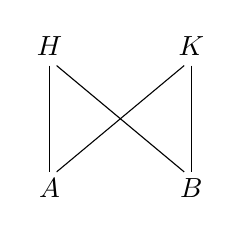
\begin{tikzpicture}[scale=0.9]
                \node [above] at (0,0) {$A$};
                \node [above] at (0,2) {$H$};
                \node [above] at (2,2) {$K$};
                \node [above] at (2,0) {$B$};
                \draw [-] (1.9,2) to (0.1,0.5);
                \draw [-] (2,2) to (2,0.5);
                \draw [-] (0,2) to (0,0.5);
                \draw [-] (0.1,2) to (1.9,0.5);
            \end{tikzpicture}
        \end{figure}
        But $A<H\cap K$, $B<H\cap K\Rightarrow A\vee B<H\cap K$. So $A\vee B\lhd H$, $A\vee B\lhd K$. That's contradictory! There is only one lower bound for $\{H,K\}$. Notice that $\{e\}<H\cap K$ so there exists at least one subgroup satisfies the condition. We have proved normality forms a lattice.
    \end{enumerate}
\end{answer}

$$ $$

\begin{ex}
    If $N_{1}\lhd G_{1}$, $N_{2}\lhd G_{2}$ then $(N_{1}\times N_{2})\lhd (G_{1}\times G_{2})$ and $(G_{1}\times G_{2})/(N_{1}\times N_{2})\cong (G_{1}/N_{1})\times(G_{2}/N_{2})$.
\end{ex}

\begin{answer}
    Take $a\in (N_{1}\times N_{2})$, $a=(n_{1},n_{2})$ where $n_{1}\in N_{1}$, $n_{2}\in N_{2}$. $\forall x\in (G_{1}\times G_{2})$, $x=(g_{1},g_{2})$ where $g_{1}\in G_{1}$, $g_{2}\in G_{2}$. $x^{-1}=(g_{1}^{-1},g_{2}^{-1})$, $x^{-1}ax=(g_{1}^{-1}n_{1}g_{1},g_{2}^{-1}n_{2}g_{2})$. $N_{1}\lhd G_{1}$, $N_{2}\lhd G_{2}$, so $g_{1}^{-1}n_{1}g_{1}\in N_{1}$, $g_{2}^{-1}n_{2}g_{2}\in N_{2}$. $x^{-1}ax\in (N_{1}\times N_{2})$. Thus $(N_{1}\times N_{2})\lhd (G_{1}\times G_{2})$.

    Assume $G_{1}=\bigcup\limits_{i\in I}N_{1}a_{i}$, $G_{2}=\bigcup\limits_{j\in J}N_{2}b_{j}$. Then $G_{1}\times G_{2}=\bigcup\limits_{i\in I}N_{1}a_{i}\times \bigcup\limits_{j\in J}N_{2}b_{j}$. Denote $A=\{a_{i}|i\in I\}$, $B=\{b_{j}|j\in J\}$. We construct two bijections $(G_{1}\times G_{2})/(N_{1}\times N_{2})\to A\times B$ and $(G_{1}/N_{1})\times(G_{2}/N_{2})$.\[f: N_{1}a_{i}\times N_{2}b_{j}\mapsto (a_{i},b_{j})\]\[g: (N_{1}a_{i}, N_{2}b_{j})\mapsto (a_{i},b_{j})\] Take $h=g^{-1}\circ f$, $f,g$ are bijections, so $h$ is an isomorphism. $(G_{1}\times G_{2})/(N_{1}\times N_{2})\cong (G_{1}/N_{1})\times(G_{2}/N_{2})$.
\end{answer}

$$ $$

\begin{ex}
    Let $N\lhd G$ and $K\lhd G$. If $N\cap K=\left\langle e\right\rangle$ and $N\vee K=G$, then $G/N\cong K$.
\end{ex}

\begin{answer}
    Assume $G=\bigcup\limits_{i\in I}Na_{i}$, we construct $f:k \to G /N$. We prove that $\forall x,y\in K$, $x,y$ belong to different cosets of $N$. Suppose not. $\exists x,y \in K$, $x,y\in Na_{i}$, then $xy^{-1}\in N\Rightarrow x=y$. That's contradictory! So $f$ is a monomorphism.

    $G=H\vee K$, so $G=HK$. we can write $x$ as $pq$, where $p\in H$, $q\in K$. $\left| G/H \right|=\left[G:H\right]=\left[HK:H\right]=\left[K:K\cap H\right]=\left| K \right| $. $f$ is a epimorphism.
    
    Thus, $G /N\cong K$.
\end{answer}

$$ $$

\begin{ex}
    If $f:G\to H$ is a homomorphism, $H$ is abelian and $N$ is a subgroup of $G$ containing $\mathrm{Ker}f$, then $N$ is normal in $G$.
\end{ex}

\begin{answer}
    Assume there exists $x\in G$, $x\notin N$ s.t. $f(x)\in f(N)$. $\exists n\in N$, $f(x)=f(n)$, $f(xn^{-1})=f(x)f(n)^{-1}=e'\Rightarrow xn^{-1}\in\mathrm{Ker}f\Rightarrow x\in N$. That's contradictory! $\forall x\in G$, $n\in N$, $f(x^{-1}nx)=f(x^{-1})f(n)f(x)=f(n)\in f(N)$, so $x^{-1}nx\in N$. Thus, $N\lhd G$.
\end{answer}

$$ $$

\begin{ex}
    \begin{enumerate}[(a)]
        \item Consider the subgroups $\left\langle 6\right\rangle$ and $\left\langle 30\right\rangle$ of $\mathbf{Z}$ and show that $\left\langle 6\right\rangle /\left\langle 30\right\rangle\cong Z_{5}$.
        \item For any $k,m>0$, $\left\langle k\right\rangle /\left\langle km\right\rangle\cong Z_{m}$; in particular, $\mathbf{Z}/\left\langle m\right\rangle=\left\langle 1\right\rangle /\left\langle m\right\rangle\cong Z_{m}$.
    \end{enumerate}
\end{ex}

\begin{answer}
    \begin{enumerate}[(a)]
        \item $\left\langle 6\right\rangle=\{6n|n\in \mathbf{Z}\}$, $\left\langle 30\right\rangle=\{30n|n\in \mathbf{Z}\}$. So $\left\langle 6\right\rangle/\left\langle 30\right\rangle=\{\left\langle 30\right\rangle, \left\langle 30\right\rangle +6, \left\langle 30\right\rangle +12, \left\langle 30\right\rangle +18, \left\langle 30\right\rangle +24\}\cong Z_{5}$
        \item $\left\langle km\right\rangle\lhd \left\langle k\right\rangle$, $\left\langle k\right\rangle=\bigcup\limits_{i\in I}(\left\langle km\right\rangle +a_{i})$. For $x\in \left\langle k\right\rangle$, $x\equiv a_{i}\mod km$, then $x\in \left\langle km \right\rangle +a_{i}$. $f:\left\langle k\right\rangle/\left\langle km\right\rangle\to \{a_{i}|i\in I\}$ defined by $f(\left\langle km\right\rangle +a_{i})=a_{i}$ is a bijection. We check that $g: \{a_{i}|i\in I\}\to Z_{m}$ is also a bijection. Define $b_{i}\equiv \frac{a_{i}}{k}\mod m$, $g(a_{i})=b_{i}$. If there exists $b_{i}=b_{j}$ for $i\neq j$, $a_{i}\equiv a_{j}\mod km$. That's contradictory! So $g$ is an injection. $g$ is obviously a surjection, so $g$ is a bijection. Take $h= g\circ f:\left\langle k\right\rangle /\left\langle km \right\rangle\to Z_{m}$ is a isomorphism, so $\left\langle k\right\rangle /\left\langle km \right\rangle\cong Z_{m}$.
    \end{enumerate}
\end{answer}

$$ $$

\begin{ex}
    If $f: G \to H$ is a homomorphism with kernel $N$ and $K<G$, then prove that $f^{-1}(f(K))=KN$. Hence $f^{-1}(f(K))=K$ if and only if $N<K$.
\end{ex}

\begin{answer}
    Take $x\in f^{-1}(f(K))$, then there exists $k\in K$ s.t. $f(x)=f(k)$. $f(xk^{-1})=f(x)f(k)^{-1}=e'\in f(K) \Rightarrow xk^{-1}\in\mathrm{Ker}f=N$. Thus, $x\in Nk\subset NK$, $f^{-1}(f(K))\subset NK$.

    $\forall x=nk\in NK$, where $n\in N$ and $k\in K$. $f(x)=f(n)f(k)=e'f(k)\in f(K)$, so $NK\subset f^{-1}(f(K))$.

    Thus, $f^{-1}(f(K))=NK$. Hence $f^{-1}(f(K))=K$ if and only if $N<K$.
\end{answer}

$$ $$

\begin{ex}
    If $N\lhd G$, $\left[G:H\right]$ finite, $H<G$, $\left| H \right| $ finite, and $\left[G:N\right]$ and $\left| H \right| $ are relatively prime, then $H<N$.
\end{ex}

\begin{answer}
    $N\lhd G\Rightarrow NH<G$. By the second isomorphism theorem, $NH /N\cong H/H\cap N\Rightarrow \left[NH:N\right]=\left[H:H\cap N\right]$. Assume $\left[G:N\right]=m$, $\left| H \right| =n$, $\left| G \right| =mnp$ where $(m,n)=1$. Then $\left| N \right| =np$, $N<NH$, assume $\left| NH \right| =knp$, $NH<G\Rightarrow knp|mnp\Rightarrow k|m$. $\left[NH:N\right]=\left[H:H\cap N\right]=k\Rightarrow k|n$. So $k=1$, $NH=N$ which means $H<N$.
\end{answer}

$$ $$

\begin{ex}
    If $N\lhd G$, $\left| N \right|$ finite, $H<G$, $\left[G:N\right] $ finite, and $\left[G:H\right]$ and $\left| N \right| $ are relatively prime, then $N<H$.
\end{ex}

\begin{answer}
    $N\lhd G\Rightarrow NH<G$. By the second isomorphism theorem, $NH /N\cong H/H\cap N\Rightarrow \left[NH:N\right]=\left[H:H\cap N\right]$. Assume $\left[G:H\right]=m$, $\left| N \right| =n$, $\left| G \right| =mnp$ where $(m,n)=1$. Then $\left| H \right| =np$, $H<NH$, assume $\left| NH \right| =knp$, $NH<G\Rightarrow knp|mnp\Rightarrow k|m$. $\left[NH:N\right]=\left[H:H\cap N\right]=kp\Rightarrow kp|np\Rightarrow k|n$. So $k=1$, $NH=H$ which means $N<H$.
\end{answer}

$$ $$

\begin{ex}
    If $H$ is a subgroup of $Z(p^{\infty})$ and $H\neq Z(p^{\infty})$, then $Z(p^{\infty}) /H\cong Z(p^{\infty})$.
\end{ex}

\begin{answer}
    From \textbf{Exercise 1.3.7}(b), we know that $H$ has the form $\left\langle \bar{\frac{1}{p^{n}}}\right\rangle$. Take $x_{i}=\bar{\frac{1}{p^{n+i}}}+H$, $x_{1}=\bar{\frac{1}{p^{n+1}}}+H$. \[\sum_{m=1}^{p}x_{1}=\bar{\frac{p}{p^{n+1}}}+pH=\bar{\frac{1}{p^{n}}}+H=H\] \[\sum_{m=1}^{p}x_{i}=\bar{\frac{p}{p^{n+i}}}+pH=\bar{\frac{1}{p^{n+i-1}}}+H=x_{i-1}\] Take $A=\{x_{i}|i\in \mathbf{Z}_{+}\}$, $\left\langle A\right\rangle\cong Z(p^{\infty})$ by \textbf{Exercise 1.3.7}(e). $\forall x\in \left\langle A\right\rangle$, $x\in Z(p^{\infty}) /H$, so $\left\langle A\right\rangle\subset Z(p^{\infty}) /H$. Take $x\in Z(p^{\infty}) /H$, $x=y+H$ where $y=\sum\limits_{i=1}^{m}\frac{a_{i}}{p^{n+i}}$, $x=\sum\limits_{i=1}^{m}(\frac{a_{i}}{p^{n+i}}+H)\in \left\langle A\right\rangle$. Thus, $Z(p^{\infty}) /H\subset \left\langle A\right\rangle$, $\left\langle A\right\rangle=Z(p^{\infty}) /H\cong Z(p^{\infty})$.
\end{answer}
\end{document}